\section{Gold-PVD}
\label{goldpvd}

Als Testsystem für PVD-Prozesse bietet sich mit kristallinem Gold ein PVD-Prozess an, der zwar durch Oberflächendiffusion dominiert wird, jedoch ideale kristalline Strukturen bildet und ausgiebig erforschte MD-Parametrisierungen vorweisen kann.
Die genutzte Parametrisierung, welche mit EAM-Potentialen arbeitet und auf Daten von Foiles et al.\cite{foiles_embedded-atom-method_1986} basiert, stammt aus dem \todo{ref}LAMMPS-Paket.
Da es sich um ein reines Metallsystem handelt, existieren ausreichend getestete EAM-Potentiale, von denen ich mich für die Nutzung der Potentiale aus der Standardbibliothek von \todo{ref}LAMMPS entschieden habe.

\subsection{Voruntersuchungen}

Zur Validierung grundlegender Materialeigenschaften wurden Bindungslängen, Dichten und Koordinationszahlen aus einer relaxierten kristallinen Phase untersucht.
Eine Stabilitätsanalyse des Precursormoleküles entfällt, da bei PVD-Prozessen nur einzelne Atome auf die Oberfläche aufgebracht werden.
Zur Bestimmung dieser Werte wurde ein Goldkristall von \SI{40x40x40}{\angstrom} Größe auf \SI{1000}{\kelvin} aufgeheizt, im kanonischen Ensemble relaxiert und anschließend abgekühlt, wobei bei den entsprechenden Temperaturen die in Tabelle \ref{tab:goldpreresults} gezeigten Werte aufgenommen.
Die Temperaturen ergeben sich aus den Umgebungsbedingungen der Literaturwerte.
Wie man den Ergebnissen ansehen kann, bleibt die Kristallstruktur erwartungsgemäß erhalten (die Schmelztemperatur wurde für die Relaxierung nicht überschritten) und stellt die Literaturwerte in guter Übereinstimmung dar.

\begin{table}[hbtp]
  %% \rowcolors{0}{white}{lightgray} 
  \caption[Eigenschaften von Gold]{Eigenschaften von Gold als Voruntersuchung des PVD-Prozesses}
  \label{tab:goldpreresults}
  \begin{tabularx}{\textwidth}{|lXXXX|}
    \hline
    \textbf{unters. Größe} & \textbf{Temperatur} & \textbf{Simulation} & \textbf{Experiment} & \textbf{Abweichung}\\
    \hline
    Bindungslänge  &  \SI{50}{\kelvin}   &  \SI{2.885}{\angstrom}                    &  \SI{2.884}{\angstrom}                    &  \SI{0.05}{\percent}  \\
    Koordination   &  \SI{50}{\kelvin}   &  \SI{12.00}{}                             &  \SI{12.00}{}                             &  \SI{0}{\percent}     \\
    Dichte         &  \SI{300}{\kelvin}  &  \SI{18.99}{\gram\per\cubic\centi\meter}  &  \SI{19.30}{\gram\per\cubic\centi\meter}  &  \SI{1.6}{\percent}   \\
    Dichte         &  \SI{500}{\kelvin}  &  \SI{18.89}{\gram\per\cubic\centi\meter}  &  \SI{19.13}{\gram\per\cubic\centi\meter}  &  \SI{1.2}{\percent}   \\
    \hline
  \end{tabularx}
\end{table}

\todo[inline]{Oberflächenvalidierung}

\subsection{Thermische Eigenschaften}

Anders als bei anderen Formulierungen bilden EAM-Potentiale zusätzlich thermische Eigenschaften von Metallen ab.
Zur Untersuchung dieser Eigenschaft wurde die Massendichte in Abhängigkeit der Temperatur für die Teststruktur untersucht, die langsam auf \SI{2000}{\kelvin}, also weit über den Schmelzpunkt von \SI{1337}{\kelvin}, aufgeheizt wurde.
Die Ergebnisse (Abbildung \ref{fig:goldthermo}) zeigen gute Übereinstimmung mit experimentellen Daten in der Temperaturabhängigkeit der Dichte sowie im Schmelzpunkt.
Für korrekte thermische Werte müssen die Relaxationszeit $t_\text{relax}$ oberhalb von ca. \SI{40}{\pico\second} und die Thermostat-Dämpfung $D_T$ im Bereich von etwa \SI{0.02}{\femto\second} liegen.

\begin{figure}[tbp]
  \centering
  \captionsetup[subfigure]{singlelinecheck=false}
  \def\subfigwidth{7cm}
  \begin{subfigure}[t]{\subfigwidth}
    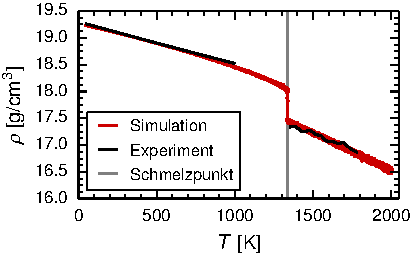
\includegraphics[width=\textwidth]{gold_bestthermo}
    \subcaption{Temperaturverlauf bei $ t_\text{relax}=\SI{50}{\pico\second}$ und $D_T=\SI{0.02}{\femto\second}$}
  \end{subfigure}
  \hfill
  \begin{subfigure}[t]{\subfigwidth}
    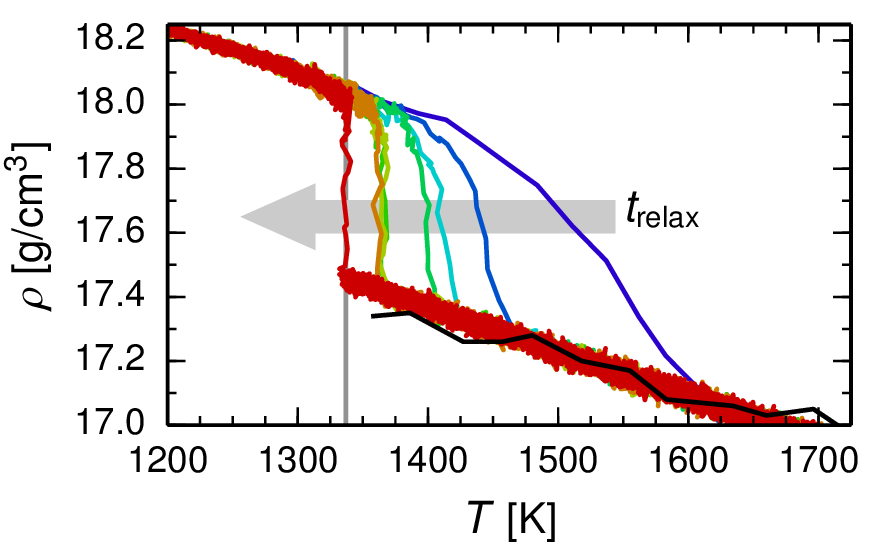
\includegraphics[width=\textwidth]{gold_relaxtime}
    \subcaption{Abhängigkeit des simulierten Schmelzpunktes von der Relaxationszeit}
  \end{subfigure}
  \caption[Ergebnisse thermischer Simulationen von Gold]{Ergebnisse thermischer Simulationen von Gold.
    Verlauf stimmt gut mit experimentellen Daten (schwarze Linien) überein.
    Experimentelle Werte stammen von aus Standardliteratur sowie von Brillo et al.\cite{brillo_density_2006}.
}
  \label{fig:goldthermo}
\end{figure}

\subsection{Prozess-Simulation}

Zur Simulation eines Gold-PVD-Prozesses mit Parsivald wurden die untersuchten Potentialparameter nebst Kristallsubstrat geladen, ein Abscheidungsmodus mit zufälligen Auftreffpositionen in der xy-Ebene gewählt und Relaxationszeiten und Reaktionsnachbarschaftsgrößen gewählt, die in den vorheringen Tests als hinreichend ermittelt wurden.
Damit ergaben sich Reaktionsräume der Größe \SI{37x37x25}{\angstrom} mit jeweils ca. 1800 Atomen, Relaxationszeiten von \SI{1.4}{\nano\second} in \SI{1400}{} Simulationsschritten und Auftreffgeschwindigkeiten von \SI{4}{\angstrom/\pico\second}, die aus üblichen Sputterbedingungen berechnet wurden.\todo{wie berechnet?}

\subsubsection{Strukturierte Substrate}

Zum Abschluss der Gold-Untersuchungen wurden strukturierte Substrate genutzt (Abbildung \ref{fig:goldsubstrate}).
Diese wurden per Materials Studio präpariert, mit Atomsk in ein kompatibles Format überführt und anschließend von Parsivald eingelesen und mit einzelnen Goldatomen im PVD-Modus beschichtet.

\begin{figure}[bt]
  \captionsetup[subfigure]{singlelinecheck=false}
  \def\subfigwidth{0.31\textwidth}
  \begin{subfigure}[t]{\subfigwidth}
    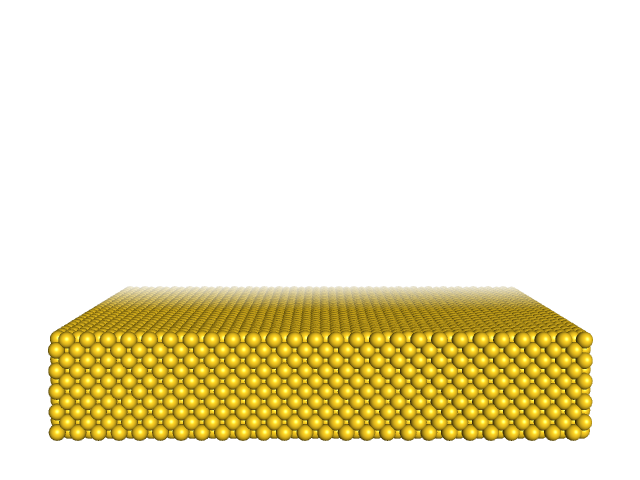
\includegraphics[width=\textwidth]{Au_substrate_flat}
    \subcaption{Flaches Gold-Substrat}
    \label{fig:goldsubstrate-a}
  \end{subfigure}
  \hfill
  \begin{subfigure}[t]{\subfigwidth}
    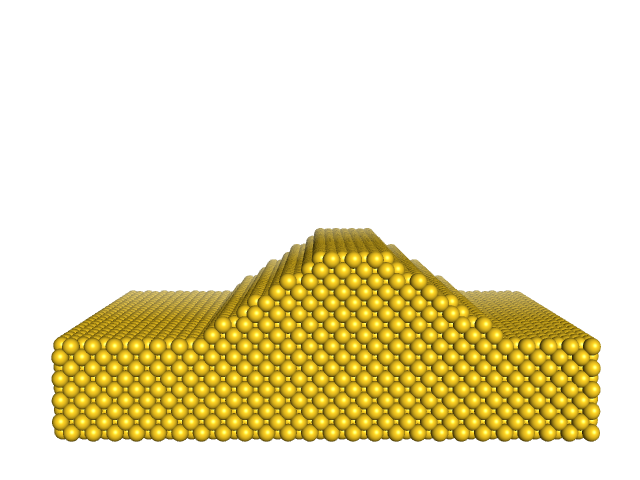
\includegraphics[width=\textwidth]{Au_substrate_step30}
    \subcaption{Gold-Stufe, 30°}
    \label{fig:goldsubstrate-b}
  \end{subfigure}
  \hfill
  \begin{subfigure}[t]{\subfigwidth}
    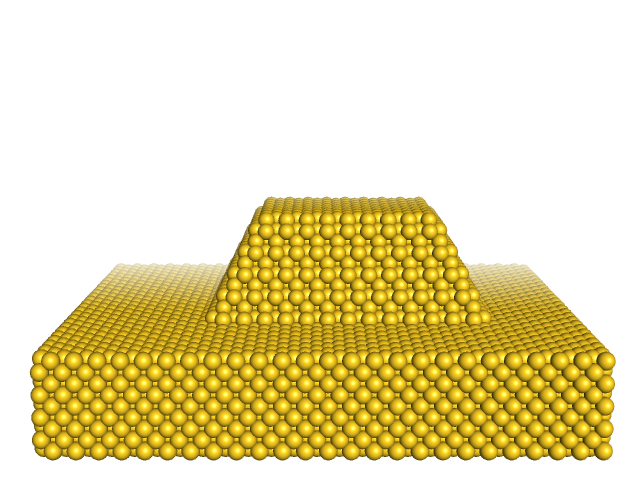
\includegraphics[width=\textwidth]{Au_substrate_tip60}
    \subcaption{Gold-Spitze, 60°}
    \label{fig:goldsubstrate-c}
  \end{subfigure}
  \caption[Strukturierte Goldsubstrate]{Goldsubstrate mit unterschiedlicher Struktur und Breite und Tiefe von \SI{100}{\angstrom}.
    Abscheidungen wurden auf flachen Substraten sowie Stufen und Spitzen mit jeweils \SI{15}{\degree}, \SI{20}{\degree}, \SI{30}{\degree}, \SI{45}{\degree}, \SI{60}{\degree} und \SI{90}{\degree} Neigung durchgeführt.}
  \label{fig:goldsubstrate}
\end{figure}

\begin{figure}[bt]
  \captionsetup[subfigure]{singlelinecheck=false}
  \def\subfigwidth{0.31\textwidth}
  \begin{subfigure}[t]{\subfigwidth}
    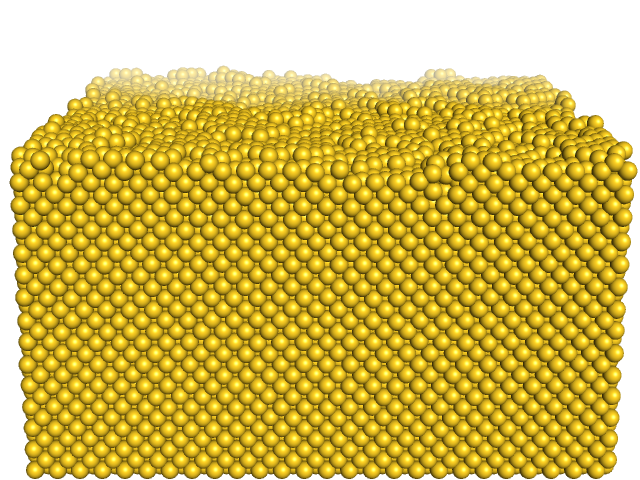
\includegraphics[width=\textwidth]{Au_deposition_flat}
    \subcaption{Abscheidung auf flachem Gold-Substrat}
    \label{fig:golddepositions-a}
  \end{subfigure}
  \hfill
  \begin{subfigure}[t]{\subfigwidth}
    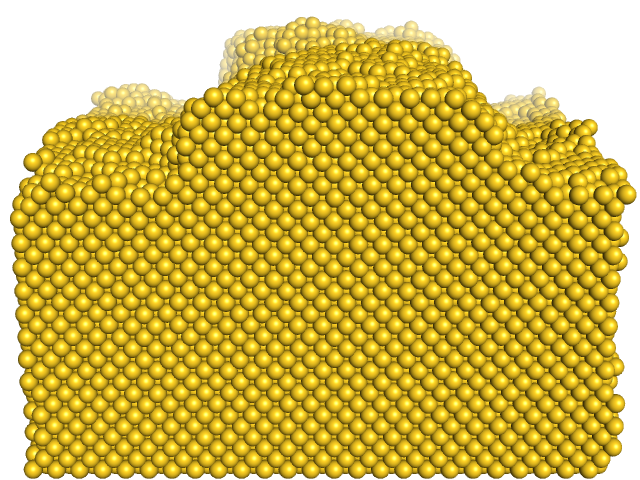
\includegraphics[width=\textwidth]{Au_deposition_step30}
    \subcaption{Abscheidung auf Gold-Stufe, \SI{30}{\degree}}
    \label{fig:golddepositions-b}
  \end{subfigure}
  \hfill
  \begin{subfigure}[t]{\subfigwidth}
    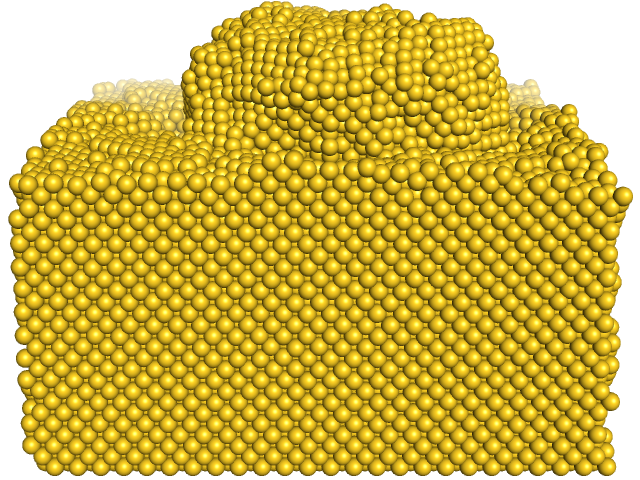
\includegraphics[width=\textwidth]{Au_deposition_tip60}
    \subcaption{Abscheidung auf Gold-Spitze, \SI{60}{\degree}}
    \label{fig:golddepositions-c}
  \end{subfigure}
  \caption[Abscheidung auf strukturierten Substraten]{
    Ergebnis der Abscheidung.
    Die Substratstruktur bleibt erkennbar, wird aber nach oben verstärkt, ansonsten aber kristallin und flach fortgesetzt.
  }
  \label{fig:golddepositions}
\end{figure}

Auf  Gold-Abscheidungen mit Parsivald (Abbildung \ref{fig:golddepositions}) zeigen perfekt fortgesetzte Kristallstrukturen, wobei die Schicht auf dem flachen Substrat nach 10 Kristallschichten eine Rauheit von einem Atomdurchmesser zeigt, die weiter beibehalten wird\todo{phrasing}.
Die strukturierten Substrate hingegen zeigen den Trend, die Neigungswinkel an Stufen und Spitzen zu verstärken.
Nach längeren Laufzeiten entstehen somit Überhänge, die durch Abschluss zu Hohlräumen führen, die sich in der Realität durch thermische Relaxation schließen.
Dahinter steht einerseits die Notwendigkeit, Gold-Atome bei Ankunft auf der Oberfläche diffundieren zu lassen, was beim aktuellen Modell nur in Grenzen angewandt wird.

Andererseits steckt dahinter ein methodischer Fehler bei Nutzung von Binning-Methoden:
Die Oberfläche wird aufgrund von Laufzeitbegrenzungen nur entlang der z-Achse bestimmt, woraufhin das neue Atom über einem Atom auf der Oberfläche platziert wird.
Das führt bei Stufen in der Struktur zu Atomen, die immer am oberen Ende einer Kante oder Neigung aufgetragen werden und dort mit statistischer Wahrscheinlichkeit verbleiben.

Eine mögliche Lösung stellt die ausführliche Parametrisierung der Oberfläche dar, beispielsweise per Alpha-Form (Abschnitt \ref{dataalphaform}, über die man die Ereigniswahrscheinlichkeit entsprechend der Einbettungsenergie variierte, angenähert über die Oberflächenkrümmung.
